\documentclass[letterpaper, 10pt, conference]{ieeeconf}
\IEEEoverridecommandlockouts
\overrideIEEEmargins

\usepackage{amsmath,amssymb,amsfonts}
\usepackage{booktabs}
\usepackage{graphicx}
\usepackage{multirow}
\usepackage{hyperref}
\usepackage{array}
\usepackage{cite}
\usepackage{xcolor}

\newcommand{\tbd}[1]{\textcolor{blue}{\texttt{[TBD: #1]}}}

\title{\LARGE \bf
Causal Mamba World-Model Guided Flow Matching for Manipulation under Transient Preconditions and Internal Occlusion
}

\author{Mingzhe Liu \textit{et al.}%
\thanks{Manuscript prepared for \textit{IEEE Robotics and Automation Letters (RA-L)} / \textit{IEEE ICRA}. Code, frozen checkpoints, and SHA256 audit manifests are archived in the project repository (\url{https://github.com/Marco6-3/World_Model}).}%
}

\begin{document}

\maketitle
\thispagestyle{empty}
\pagestyle{empty}

\begin{abstract}
Generative visuomotor policies based on Diffusion and Conditional Flow Matching (CFM) excel at quasi-static imitation, yet struggle in contact-rich manipulation tasks governed by \emph{transient preconditions}---such as inserting objects into spring-loaded containers or elastic-mouthed bags whose apertures can collapse mid-execution---and \emph{internal visual occlusion}, where previously packed items disappear from view over long horizons. Simply co-generating future states alongside actions induces severe state hallucination ($90.0\%$ false-safe collision predictions in closed loop), whereas post-hoc world-model ranking or endpoint optimization (e.g., Generative Predictive Control, GPC) either fails when recovery demonstrations are scarce in the policy prior or incurs prohibitive optimization latency ($\sim 0.78\text{ s}$) relative to sub-second closure windows ($0.10\text{--}0.27\text{ s}$). We propose \textbf{Causal Mamba World-Model Guided Flow Matching}, a unified framework pairing a $256\text{D}$ past-to-future Selective State-Space World Model (\texttt{Mamba-Past} and \texttt{Mamba-Future}) with split-conformal clearance calibration and risk-adaptive late-stage in-flow causal guidance ($\tau_{\text{start}} \in [0.7, 0.9]$). Across a three-stage simulation benchmark suite---public \texttt{Push-T} ($50$ seeds), \texttt{Spring-Lid} mechanism diagnostics, and flagship bimanual dynamic \texttt{Bag-Packing} under $15\%$ scarce recovery priors---our framework: (i) retains occluded slot occupancy across $>14\text{ s}$ horizons ($100.0\%$ closed-loop second-slot routing vs.\ $50.0\%$ chance performance for short-history baselines); (ii) compresses world-model clearance error to $4.57\text{ mm}$ ($0.9\%$ collision miss rate at $256\text{D}$ vs.\ $70.7\%$ at $4\text{D}$); and (iii) achieves $18/18$ ($100.0\%$) zero-collision recovery from mid-insertion collar slip in paused-physics evaluation, outperforming \texttt{GPC-RANK} ($0/18$), \texttt{4D-WM} ($0/18$), and \texttt{GPC-OPT} ($1/18$). Furthermore, parallel associative SSM scans and static-buffer CUDA Graph capture compress full guided latency from $111.35\text{--}182.75\text{ ms}$ down to $13.51\text{--}17.15\text{ ms}$ ($<1$ tick at $30\text{ Hz}$), preserving $18/18$ ($100.0\%$) nominal packing and boosting strict zero-collision slip recovery by $2.6\times\text{--}4.0\times$ ($13/18$ vs.\ $5/18$ at $\tau=0.7$; $0/18$ no-timeout recovery for all baselines) under \emph{unpaused wall-clock asynchronous physics}. Finally, we establish a single-arm real-robot validation protocol (\texttt{Stage D}) for physical hardware verification.
\end{abstract}

% ============================================================================
\section{Introduction}
% ============================================================================

Deploying learned manipulation policies in unstructured physical environments requires reasoning beyond instantaneous geometry. Consider packing multiple heterogeneous items into an opaque spring-lid bin or an elastic-collared deformable bag (Fig.~\ref{fig:flagship}). Although the aperture is open when the robot initiates insertion at time $t$ (clearance $d_{\text{clear},t} > d_{\text{safe}}$), external restoring dynamics---such as unknown hinge stiffness $\xi \in \{\text{static}, \text{slow}, \text{fast}\}$ or sudden support-hand slip (\texttt{Collar-Slip})---can collapse the passage within $0.10\text{--}0.27\text{ s}$, well before an $H$-step action chunk completes execution. Meanwhile, once the first item settles inside the opaque container, it becomes visually occluded over the subsequent $5\text{--}10\text{ s}$ pickup-and-transport cycle of the second item.

\begin{figure*}[t]
    \centering
    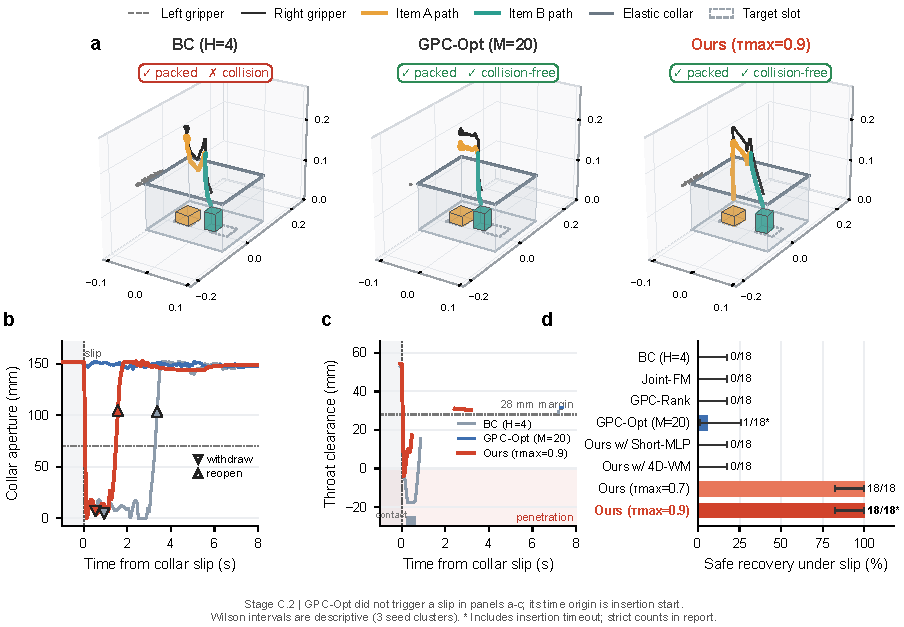
\includegraphics[width=0.96\textwidth]{../outputs/stage_c_bag/paper/fig_stage_c_bag.pdf}
    \caption{Flagship Stage C.2 bimanual dynamic bag-packing under internal occlusion and mid-insertion \texttt{Collar-Slip} (\texttt{elastic\_fast}, seed $2000$). Short-history \texttt{BC H4} forgets the occluded first item's slot ($50\%$ routing) and collides upon slip ($0/18$ safe recovery); \texttt{GPC-OPT} stalls under iterative post-hoc optimization ($776.96\text{ ms}$, $1/18$ safe recovery); \textbf{Ours (\texttt{256D} Causal Mamba + Split-Conformal Late-Stage In-Flow Guidance)} remembers the occupied slot ($18/18$) and executes zero-collision withdrawal, collar re-spreading, and re-insertion ($18/18$ safe recovery).}
    \label{fig:flagship}
\end{figure*}

Standard action-chunking generative policies, including ACT~\cite{zhao2023act}, Diffusion Policy~\cite{chi2024diffusion}, and Conditional Flow Matching (CFM)~\cite{lipman2023flow}, face three structural bottlenecks in this regime:
\begin{enumerate}
    \item \textbf{Execution Memory Loss under Internal Occlusion:} Short sliding observation windows ($L = 2\text{--}4$ frames) discard pre-blackout visual evidence once transport duration exceeds $L\Delta t$, reducing multi-item slot assignment to a $50\%$ blind guess and losing latent stiffness cues during contact handoffs.
    \item \textbf{State Hallucination in Joint State-Action Generation:} Co-denoising actions and future safety states $X_\tau = (A_\tau, S_\tau)$ under risk gradients $-\eta \nabla_{X_\tau} \mathcal{J}(S_\tau)$~\cite{janner2022diffuser} decouples predicted safety from physical causality ($\nabla_{A_\tau}\mathcal{J}(S_\tau) = 0$). In our closed-loop audit, joint guidance falsifies its own predicted impulse below the collision threshold in $90.0\%$ ($9/10$) of actual physical pinch events.
    \item \textbf{Prior Scarcity vs.\ Wall-Clock Latency in Post-Hoc Planning:} Test-time world-model planners such as Generative Predictive Control (\texttt{GPC-RANK} and \texttt{GPC-OPT})~\cite{qi2026gpc} evaluate completed policy samples at $\tau = 1.0$. While effective when expert priors densely cover target behaviors, emergency mid-flight withdrawal demonstrations are inherently \emph{scarce} in real datasets. Under a $15\%$ recovery prior, \texttt{GPC-RANK} fails to sample collision-free withdrawals even at $K=16$, whereas \texttt{GPC-OPT} ($M=20$ backpropagation passes) incurs $\sim 777\text{ ms}$ latency---exceeding sub-second closure windows---and risks off-manifold drift.
\end{enumerate}

To address these challenges within a unified, rigorously audited scope, we propose \textbf{Causal Mamba World-Model Guided Flow Matching}. Our main contributions are:
\begin{itemize}
    \item \textbf{Unified Past-to-Future \texttt{256D} Mamba World Model:} We pair a selective state-space history encoder (\texttt{Mamba-Past}) compressing $64$-token ($\sim 14.8\text{ s}$) histories into $b_t \in \mathbb{R}^{256}$ for occluded slot and regime inference with an action-conditioned \texttt{Mamba-Future} rollout backbone and decoupled state/safety readouts. Scaling future dynamics from $4\text{D}$ safety scalars to $256\text{D}$ reduces spring-lid collision miss rates from $70.7\%$ to $0.9\%$ and bag clearance MAE from $10.84\text{ mm}$ to $4.57\text{ mm}$.
    \item \textbf{Split-Conformal Clearance Calibration \& Risk-Adaptive In-Flow Guidance:} Using one-step Euler extrapolation $\hat{A}_1(A_\tau, \tau)$ at $\tau_{\text{start}} \in [0.7, 0.9]$, we evaluate causal risk over split-conformal lower clearance bounds $\underline{d}_{\text{clear}} = \hat{d}_{\text{clear}} - \hat{q}_{1-\alpha}$, occupancy gating, and terminal clearance extrapolation. Early steps ($\tau < \tau_{\text{start}}$) remain world-model-free to preserve manifold smoothness, while risk-adaptive late-stage Jacobian guidance steers trajectories out of scarce-prior danger zones $7.0\times$ faster than \texttt{GPC-OPT}.
    \item \textbf{Mechanistic Regime Delineation \& Three-Stage Simulation + Real-Robot Protocol:} Across \texttt{Push-T}, \texttt{Spring-Lid}, and \texttt{Bag-Packing}, we isolate dense-prior ranking vs.\ scarce-prior in-flow guidance (boosting paired physical collision-free withdrawal from $50.0\%$ to $100.0\%$ under identical $256\text{D}$ world models and particle budgets $K$), alongside a hardware-ready wall-clock single-arm real-robot protocol (\texttt{Stage D}).
\end{itemize}

% ============================================================================
\section{Related Work}
% ============================================================================

\subsection{Generative Imitation and Test-Time Guidance}
Diffusion Policy~\cite{chi2024diffusion} and flow-matching policies~\cite{lipman2023flow, black2024pi0} model multi-modal action chunks via iterative integration. Test-time guidance methods~\cite{janner2022diffuser, xiao2025safediffuser} inject cost gradients during generation, yet assume either analytical obstacle geometry or joint state-action generation~\cite{janner2022diffuser}, which suffers from state hallucination. Moreover, guiding from $\tau=0$ incurs $\mathcal{O}((1-\tau)^2)$ endpoint extrapolation error on noisy samples, motivating our late-stage ($\tau_{\text{start}} \in [0.7, 0.9]$) causal intervention.

\subsection{Action-Conditioned World Models for Manipulation}
Forward dynamics models trained on mixed expert and exploratory trajectories enable counterfactual planning~\cite{hafner2025dreamerv3, zhou2025dinowm, qi2026gpc}. Most closely related, GPC~\cite{qi2026gpc} enhances frozen policies via $\tau=1.0$ sample ranking (\texttt{GPC-RANK}) or endpoint optimization (\texttt{GPC-OPT}). We advance beyond GPC via: (i) \texttt{Mamba-Past} selective long-horizon memory for internal occlusion; (ii) in-flow causal Jacobian guidance under scarce recovery priors; and (iii) split-conformal clearance calibration.

\subsection{Selective State Spaces and Conformal Safety}
Mamba~\cite{gu2024mamba} achieves linear-time sequence modeling with input-dependent selection gates $(\Delta_t, B_t, C_t)$ that latch sparse transient events across hundreds of quasi-static frames. Split Conformal Prediction~\cite{angelopoulos2023conformal, lindemann2023conformal} provides distribution-free finite-sample error bounds; here we calibrate action-conditioned clearance overestimation across multi-modal restoring dynamics to gate in-flow insertion and withdrawal.

% ============================================================================
\section{Problem Formulation and Failure Diagnostics}
% ============================================================================

At discrete step $t$ ($\Delta t = 33.3\text{ ms}$), the robot receives $o_t \in \mathbb{R}^{D_o}$ containing proprioception, aperture geometry, and visible object poses (masked to zero below container occlusion height $z_{\text{occ}}$), while the aperture evolves under latent dynamics $\xi \in \{1, \dots, M\}$. Given candidate clean action chunk $A_1 = a_{t:t+H-1} \in \mathbb{R}^{H \times D_a}$, future safety coordinates at $t+k$ are:
\begin{equation}
    s_{t+k} = \big[d_{\text{clear}, t+k},\; \phi_{\text{occ}, t+k},\; p_{\text{prog}, t+k},\; c_{\text{col}, t+k}\big]^\top,
\end{equation}
denoting 3D effective clearance $d_{\text{clear}}$, channel occupancy $\phi_{\text{occ}} \in [0,1]$, insertion progress $p_{\text{prog}} \in [0,1]$, and unintended contact impulse $c_{\text{col}} \ge 0$.

Iterative diagnostics expose three failure modes of naive baselines: (i) flat MLPs with white noise exhibit $52.6\text{ mm}$ median inter-step jumps ($0\%$ success), necessitating \texttt{1D-Conv} residual blocks, correlated temporal noise, and $7.5\text{ mm/step}$ kinematic limits; (ii) co-generating $X_\tau = (A_\tau, S_\tau)$ allows $-\nabla_{S_\tau}\mathcal{J}(S_\tau)$ to falsify predicted impulse in $9/10$ physical collisions, requiring strict causal parameterization $S = W_\psi(b_t, A_1, \xi)$; and (iii) un-gated clearance penalties penalize post-withdrawal lid closure, requiring $\phi_{\text{occ}}$ gating and terminal closure-rate extrapolation to overcome horizon myopia ($H\Delta t = 0.80\text{ s} < 0.933\text{ s}$ slow closure).

% ============================================================================
\section{Methodology}
% ============================================================================

\subsection{Unified Past-to-Future \texttt{256D} Mamba World Model}
\subsubsection{Long-Horizon Occlusion Memory (\texttt{Mamba-Past})}
Given a $64$-token multi-scale history $\mathbf{o}_t = (o_{t_1}, \dots, o_{t_{64}})$ spanning $444$ frames ($\approx 14.8\text{ s}$; $60$ strided context tokens plus $4$ consecutive recent frames), \texttt{Mamba-Past} applies causal depthwise \texttt{1D-Conv} and selective SSM recurrence ($D_z = 256$):
\begin{equation}
    h_j = \exp(\Delta_j A) \odot h_{j-1} + (\Delta_j \odot x_j) B_j^\top, \quad y_j = h_j C_j + D \odot x_j,
\end{equation}
producing terminal belief $b_t \in \mathbb{R}^{256}$, dynamics posterior $\hat{p}(\xi \mid b_t) = \text{Softmax}(W_\xi b_t)$, and occluded slot occupancy $\hat{q}_{\text{slot}}(b_t) = \sigma(W_{\text{slot}} b_t) \in [0,1]^2$.

\subsubsection{Action-Conditioned Rollout (\texttt{Mamba-Future})}
Initialized at $z_t(\xi) = \tanh(W_{\text{init}}[b_t; e_\xi; c_{\text{stage}}])$, \texttt{Mamba-Future} rolls out $H=24$ latent states strictly conditioned on clean action proposal $\hat{A}_1$:
\begin{equation}
    \hat{z}_{t+k}(\xi) = \text{Mamba}_{\text{future}}\!\big(W_a \hat{a}_{t+k-1} + z_t(\xi) + W_{\text{fb}} \hat{z}_{t+k-1}(\xi)\big).
\end{equation}
Two decoupled MLP heads supervise $\hat{z}_{t+k} \in \mathbb{R}^{256}$: a geometric state head $g_{\text{state}}(\hat{z}_{t+k})$ preserving full rigid-body kinematics, and a structured safety head $g_{\text{safe}}(\hat{z}_{t+k})$ predicting $[\hat{d}_{\text{clear}}, \hat{\phi}_{\text{occ}}, \hat{p}_{\text{prog}}, \hat{c}_{\text{col}}]^\top$.

\subsection{Split-Conformal Clearance Calibration \& Causal Risk}
On validation samples $i \in \{1, \dots, N_{\text{cal}}\}$ with posterior-mean predicted clearance $\bar{d}_{\text{clear},i,k}$, we compute simultaneous horizon overestimation scores and the $(1-\alpha)$ quantile ($\alpha=0.10$):
\begin{equation}
    s_i = \max_{1 \le k \le H} \big(\bar{d}_{\text{clear},i,k} - d_{\text{clear},i,k}\big), \quad \hat{q}_{1-\alpha} = \text{Quantile}_{\frac{\lceil(N_{\text{cal}}+1)(1-\alpha)\rceil}{N_{\text{cal}}}}(\{s_i\}).
\end{equation}
Substituting $\underline{d}_{\text{clear},k}(\xi) = \hat{d}_{\text{clear},k}(\xi) - \hat{q}_{1-\alpha}$ and conformal gate $g_{\text{safe},k} = \sigma((\underline{d}_{\text{clear},k} - d_{\text{gate}})/\kappa_g)$ (zeroed under collapse), the regime risk is:
\begin{align}
    \mathcal{J}(\hat{A}_1; \xi) &= \frac{1}{H}\sum_{k=1}^H \Big[\lambda_{\text{pinch}}\hat{\phi}_{\text{occ},k}\big[d_{\text{margin}} - \underline{d}_{\text{clear},k}\big]_+^2 + \lambda_{\text{imp}}\hat{c}_{\text{col},k} \nonumber \\
    &\quad - \lambda_{\text{prog}} g_{\text{safe},k}\hat{p}_{\text{prog},k} + \Psi_{\text{task}}(\hat{a}_{t+k-1}, \text{sg}[g_{\text{safe},k}])\Big] \nonumber \\
    &\quad + \lambda_{\text{term}}\big[d_{\text{term}} - \underline{d}_{\text{proj}}\big]_+^2,
\end{align}
where $\text{sg}[\cdot]$ prevents lowering predicted clearance to disable insertion potentials, and $\underline{d}_{\text{proj}} = \underline{d}_{\text{clear},H} - \dot{d}_{\text{close}} T_{\text{rem}}(1 - \hat{p}_{\text{prog},H})$. Total expected risk is $\mathcal{R}(\hat{A}_1) = \sum_\xi \hat{p}(\xi \mid b_t)\mathcal{J}(\hat{A}_1;\xi) + \mathcal{J}_{\text{slot}}(\hat{A}_1, \hat{q}_{\text{slot}}(b_t))$.

\subsection{Risk-Adaptive Late-Stage In-Flow Guidance}
Given frozen CFM field $v_\theta(A_\tau, \tau \mid \mathbf{o}_{t,\text{short}}, \hat{h}_{\text{slot}})$ and $K$ correlated Gaussian noise particles over $S=10$ Euler steps: (i) for $\tau \in [0, 0.7)$, particles integrate $v_\theta$ without world-model calls; (ii) at $\tau = 0.7$, one-step extrapolation $\hat{A}_1^{(k)} = A_{0.7}^{(k)} + 0.3 v_\theta(A_{0.7}^{(k)}, 0.7)$ inspects $\underline{d}_{\min}$, adaptively advancing $\tau_{\text{actual}} \leftarrow 0.7$ with emergency gain $\eta_{\text{emerg}}$ whenever $\underline{d}_{\min} < 18\text{ mm}$ or rapid aperture drop occurs; (iii) at $\tau = \tau_{\text{actual}}$, the minimum-risk particle $k^\star$ is retained and refined for $\tau \in [\tau_{\text{actual}}, 1.0]$ via normalized causal gradients:
\begin{equation}
    A_{\tau+\Delta\tau} = A_\tau + \Delta\tau\Big[v_\theta(A_\tau,\tau) - \eta_{\text{ada}}\Gamma\!\big(\nabla_{A_\tau}\mathcal{R}(A_\tau + (1-\tau)v_\theta)\big)\Big].
\end{equation}

% ============================================================================
\section{Experimental Evaluation}
% ============================================================================

\subsection{Stage A: Public \texttt{Push-T} Benchmark \& Intervention Timing}
Across $50$ paired seeds (\texttt{10000--10049}) on \texttt{gym-pusht}~\cite{chi2024diffusion} using a shared frozen $256$-channel \texttt{PushTFlow} and $128\text{D}$ Mamba world model (Table~\ref{tab:pusht}), early guidance ($\tau_{\text{start}}=0.0$) degrades IoU below \texttt{BC} ($0.667$ vs.\ $0.681$) due to noisy endpoint extrapolation. Delaying intervention to $\tau_{\text{start}}=0.9$ reaches $0.824$ IoU ($28/50$ successes), matching \texttt{GPC-RANK+OPT} ($0.825$, $29/50$) at $6.7\times$ lower isolated GPU latency ($72.4\text{ ms}$ vs.\ $485.9\text{ ms}$). Under \texttt{Push-T}'s dense expert coverage, large-sample ranking (\texttt{GPC-RANK} $K=64$) reaches $0.851$ IoU; however, as shown in Stage C.2, pure ranking collapses when safety recovery demonstrations are scarce.

\begin{table}[t]
\centering
\caption{Public \texttt{Push-T} Benchmark ($50$ Paired Test Seeds, RTX 5060)}
\label{tab:pusht}
\setlength{\tabcolsep}{3.5pt}
\begin{tabular}{lcccccc}
\toprule
Method & $K$ & $M$ & $\tau_{\text{start}}$ & Final IoU $\uparrow$ & Success $\uparrow$ & P50 (ms) $\downarrow$ \\
\midrule
\texttt{BC} (Frozen CFM) & 1 & 0 & --- & 0.681 & 12/50 & 26.5 \\
Early In-Flow & 8 & 0 & 0.0 & 0.667 & 14/50 & 341.8 \\
Mid In-Flow & 8 & 0 & 0.5 & 0.780 & 20/50 & 190.6 \\
\textbf{Ours ($\tau=0.7$)} & 8 & 0 & 0.7 & 0.766 & 23/50 & 134.6 \\
\textbf{Ours ($\tau=0.9$)} & 8 & 0 & 0.9 & \textbf{0.824} & \textbf{28/50} & \textbf{72.4} \\
Endpoint Rank ($K=8$) & 8 & 0 & 1.0 & 0.792 & 25/50 & 40.8 \\
\texttt{GPC-RANK} ($K=16$) & 16 & 0 & 1.0 & 0.803 & 28/50 & 45.2 \\
\texttt{GPC-RANK} ($K=64$) & 64 & 0 & 1.0 & \textbf{0.851} & 25/50 & 85.4 \\
\texttt{GPC-OPT} ($M=20$) & 1 & 20 & 1.0 & 0.785 & 21/50 & 583.4 \\
\texttt{GPC-RANK+OPT} & 8 & 15 & 1.0 & 0.825 & \textbf{29/50} & 485.9 \\
\bottomrule
\end{tabular}
\end{table}

\subsection{Stage B: \texttt{Spring-Lid} Mechanism \& Latent Dimension Scaling}
On the IsaacLab/PhysX bimanual \texttt{Spring-Lid} bench: (i) closed-loop auditing confirms that \texttt{Joint-FM} predicts collision-free impulse ($<0.004\text{ N}\cdot\text{s}$) in $9/10$ ($90.0\%$) of actual physical pinch prefixes; (ii) under $24$-frame handoff occlusion, \texttt{Short-MLP (H=4)} drops to $36.4\%$ regime accuracy (lid MAE $0.347\text{ rad}$), whereas \texttt{Mamba-Past} achieves $100.0\%$ accuracy and lowest lid MAE ($0.083\text{ rad}$); and (iii) scaling $D_z$ from $4\text{D}$ to $256\text{D}$ (Table~\ref{tab:spring_dim}) cuts collision miss rates from $70.7\%$ ($4949/7000$) to $0.9\%$ ($63/7000$) and uniquely achieves $6/6$ ($100\%$) offline safe branch ranking.

\begin{table}[t]
\centering
\caption{\texttt{Spring-Lid} Latent Dimension Scaling ($2040$ Held-Out Windows)}
\label{tab:spring_dim}
\setlength{\tabcolsep}{3.5pt}
\begin{tabular}{ccccc}
\toprule
Latent $D_z$ & Clear. MAE (mm) & Obj. MAE (mm) & Miss Rate $\downarrow$ & Safe Rank $\uparrow$ \\
\midrule
$4\text{D}$ & 11.69 & 26.54 & 70.7\% & 2/6 \\
$32\text{D}$ & 5.48 & 5.64 & 2.6\% & 4/6 \\
$128\text{D}$ & \textbf{4.16} & 3.65 & 1.4\% & 4/6 \\
\textbf{$256\text{D}$ (Ours)} & 4.78 & \textbf{3.03} & \textbf{0.9\%} & \textbf{6/6} \\
\bottomrule
\end{tabular}
\end{table}

\subsection{Stage C.2: Bimanual Dynamic Bag-Packing (Scarce Prior)}
In \texttt{Bag-Packing}, the robot packs \texttt{ItemA} and \texttt{ItemB} into left/right occluded slots across \texttt{relaxed}, \texttt{elastic\_slow} ($0.267\text{ s}$), and \texttt{elastic\_fast} ($0.100\text{ s}$ retraction) modes under a $15\%$ scarce recovery prior ($168/1152$ recovery windows retained for \texttt{BagFlow}/\texttt{Joint-FM}).

\texttt{Full 256D Mamba} achieves $4.57\text{ mm}$ clearance MAE, $95.3\%$ handoff occluded-slot readout ($100.0\%$ on $438$ balanced memory-probe samples vs.\ $50.0\%$ for \texttt{Short-MLP H4}), and a tight $90\%$ conformal quantile $\hat{q}_{0.90} = 10.50\text{ mm}$ (vs.\ $24.89\text{ mm}$ for \texttt{4D-WM}, MAE $10.84\text{ mm}$). In closed-loop evaluation (Table~\ref{tab:bag_main}), all \texttt{H4} baselines degrade to $9/18$ ($50.0\%$) second-slot routing, while \textbf{Ours ($\tau=0.7$ and $\tau=0.9$)} achieves $18/18$ ($100\%$) nominal packing and $18/18$ ($100\%$) zero-collision slip recovery ($7.0\times$ faster than \texttt{GPC-OPT}). Crucially, even when \texttt{GPC-RANK} shares the exact same \texttt{Full 256D} world model on all $12$ held-out post-slip states, scaling $K=2 \to 16$ plateaus at $6/12$ ($50.0\%$) collision-free withdrawal, whereas \textbf{Ours} achieves $12/12$ ($100.0\%$) across all $K \in \{2,4,8,16\}$.

\begin{table*}[t]
\centering
\caption{Stage C.2 Bimanual Dynamic Bag-Packing Closed-Loop Evaluation ($N=18$ Paired Episodes / Method)}
\label{tab:bag_main}
\begin{tabular}{lccccccc}
\toprule
& \multicolumn{3}{c}{\textbf{Table C1: Nominal Occluded Dual-Item Packing}} & \multicolumn{3}{c}{\textbf{Table C2: Mid-Insertion \texttt{Collar-Slip} Perturbation}} & \\
\cmidrule(lr){2-4} \cmidrule(lr){5-7}
Method & Dual Success $\uparrow$ & 2nd-Slot Correct $\uparrow$ & Collisions $\downarrow$ & Pre-Withdraw Graze $\downarrow$ & Safe Recovery $\uparrow$ & Safe (No Timeout) $\uparrow$ & P50: Eager $\to$ Graph (ms) $\downarrow$ \\
\midrule
\texttt{BC H4} ($K=1$) & 12/18 & 9/18 (50.0\%) & 9/18 & 18/18 & 0/18 (0.0\%) & 0/18 (0.0\%) & 19.76 $\to$ \textbf{4.02} \\
\texttt{Joint-FM} & 4/18 & 9/18 (50.0\%) & 6/18 & 8/18 & 0/18 (0.0\%) & 0/18 (0.0\%) & 33.12 $\to$ \textbf{3.92} \\
\texttt{GPC-RANK} ($K=16$, \texttt{H4}) & 9/18 & 9/18 (50.0\%) & 9/18 & 12/18 & 0/18 (0.0\%) & 0/18 (0.0\%) & 34.48 $\to$ 6.18 \\
\texttt{GPC-OPT} ($M=20$, \texttt{H4}) & 6/18 & 9/18 (50.0\%) & 3/18 & 0/6 trig. & 1/18 (5.6\%) & 0/18 (0.0\%) & 776.96 $\to$ 69.17 \\
\texttt{Ours Short-MLP H4} & 3/18 & 9/18 (50.0\%) & 6/18 & \textbf{0/18} & 0/18 (0.0\%) & 0/18 (0.0\%) & 173.45 $\to$ 17.11 \\
\texttt{Ours 4D-WM} & 16/18 & \textbf{18/18 (100\%)} & \textbf{0/18} & 18/18 & 0/18 (0.0\%) & 0/18 (0.0\%) & 84.41 $\to$ 8.05 \\
\textbf{\texttt{Ours (256D, $\tau=0.7$)}} & \textbf{18/18 (100\%)} & \textbf{18/18 (100\%)} & \textbf{0/18} & \textbf{0/18} & \textbf{18/18 (100\%)} & \textbf{18/18 (100\%)} & 182.75 $\to$ \textbf{17.15} \\
\textbf{\texttt{Ours (256D, $\tau=0.9$)}} & \textbf{18/18 (100\%)} & \textbf{18/18 (100\%)} & \textbf{0/18} & \textbf{0/18} & \textbf{18/18 (100\%)} & \textbf{17/18 (94.4\%)} & 111.35 $\to$ \textbf{13.51} \\
\bottomrule
\end{tabular}
\end{table*}

\subsection{Sub-Tick Acceleration \& Unpaused Wall-Clock Audit}
Without retraining frozen Stage C.2 checkpoints ($0/192$ slot/$\tau$ discrepancies, max action diff $\le 4.13\times 10^{-5}\text{ m}$), replacing sequential Python SSM scans with Hillis--Steele parallel associative scans and static-buffer \texttt{CUDAGraphPlanner} capture cuts isolated GPU P50 latency to $\mathbf{13.51\text{ ms}}$ ($8.24\times$, \texttt{$\tau=0.9$}) and $\mathbf{17.15\text{ ms}}$ ($10.66\times$, \texttt{$\tau=0.7$})---strictly within one $30\text{ Hz}$ tick ($\Delta k = 1$, $33.33\text{ ms}$), whereas \texttt{GPC-OPT} still requires $69.17\text{ ms}$ ($\Delta k = 3$; $996.59\text{ ms}$ eager). Evaluating $342$ audited episodes under \textbf{unpaused wall-clock physics} (\texttt{--wall-clock}, advancing $\Delta k = \max(1,\lceil \Delta t_{\text{infer}}/\Delta t_{\text{ctrl}}\rceil)$ PhysX steps during inference with chunk-offset alignment \texttt{actions[min($\Delta k$,H-1):]}):
\begin{itemize}
    \item \textbf{Nominal Wall-Clock Packing:} Both \texttt{Ours ($\tau=0.7, 0.9$)} achieve $\mathbf{18/18}$ ($100\%$) dual-item success, $\mathbf{18/18}$ ($100\%$) occluded second-slot routing, and $\mathbf{0/18}$ collisions ($14.45\text{--}18.07\text{ ms}$ closed-loop P50, $\Delta k=1$), vs.\ $9/18$ ($50\%$) routing for all \texttt{H4} baselines and $1/18$ ($5.6\%$) success for \texttt{GPC-OPT}.
    \item \textbf{Wall-Clock \texttt{Collar-Slip} \& Multi-Tick Lag Ablation:} Disabling CUDA Graph (\texttt{--no-cuda-graph}, $\sim 158\text{ ms}$, $\Delta k = 5$ ticks $> 100\text{ ms}$ \texttt{elastic\_fast} closure) collapses strict zero-collision recovery to $5/18$ (\texttt{$\tau=0.7$}), $3/18$ (\texttt{$\tau=0.9$}), and $0/18$ for eager \texttt{GPC-OPT} ($\Delta k=25$, $18/18$ collisions). Restoring sub-tick execution ($\Delta k=1$, $17.77\text{ ms}$) preserves $\mathbf{18/18}$ ($100\%$) dual-item completion and boosts strict zero-collision recovery by $\mathbf{2.6\times\text{--}4.0\times}$ to $\mathbf{13/18}$ ($72.2\%$, $0$ timeouts for \texttt{$\tau=0.7$}; $12/18$ for \texttt{$\tau=0.9$}), whereas all six baselines achieve $\mathbf{0/18}$ ($0.0\%$) no-timeout safe recovery.
\end{itemize}
Remaining pre-submission items include pure state-risk Jacobian ablation ($\Psi_{\text{task}} \equiv 0$, \tbd{X/48}), episode-level conformal calibration ($N_{\text{cal}} \ge 30$, \tbd{$\ge 90\%$}), and \textbf{Stage D Single-Arm Real-Robot Validation} on an RGB-D-equipped 6-DoF arm (UR5) with an opaque dual-slot elastic/spring container:
\begin{itemize}
    \item \textbf{Exp.\ R1 (Occluded Dual-Item Routing, $10$ trials/method):} \texttt{Ours} vs.\ \texttt{BC H4} (\tbd{target $10/10$ vs.\ $\sim 5/10$}).
    \item \textbf{Exp.\ R2 (Wall-Clock Mid-Insertion Retraction, $10$ trials/method):} Real-time withdrawal (\tbd{$<30\text{ ms}$, $\ge 9/10$ safe recovery}) vs.\ \texttt{GPC-OPT} (\tbd{$\sim 800\text{ ms}$}).
\end{itemize}

% ============================================================================
\section{Limitations and Conclusion}
% ============================================================================

Simulation bag elasticity uses coupled rigid-lip spring-dampers rather than cloth FEM, motivating physical fabric evaluation in Stage D; sliding-window conformal scores require episode-level sampling for strict exchangeability; and local in-flow gradients still rely on minimal ($\sim 15\%$) multi-modal recovery support. Overall, uniting a $256\text{D}$ past-to-future Mamba world model with split-conformal risk-adaptive late-stage flow guidance resolves internal occlusion, eliminates joint-generation state hallucinations, and enables real-time collision-free recovery under transient preconditions.

\begin{thebibliography}{99}
\bibitem{zhao2023act} T. Z. Zhao, V. Kumar, S. Levine, and C. Finn, ``Learning fine-grained bimanual manipulation with low-cost hardware,'' in \textit{Proc. RSS}, 2023.
\bibitem{chi2024diffusion} C. Chi \textit{et al.}, ``Diffusion policy: Visuomotor policy learning via action diffusion,'' \textit{IJRR}, 2024.
\bibitem{lipman2023flow} Y. Lipman \textit{et al.}, ``Flow matching for generative modeling,'' in \textit{Proc. ICLR}, 2023.
\bibitem{janner2022diffuser} M. Janner, Y. Du, J. B. Tenenbaum, and S. Levine, ``Planning with diffusion for flexible behavior synthesis,'' in \textit{Proc. ICML}, 2022.
\bibitem{qi2026gpc} A. Qi \textit{et al.}, ``Generative predictive control: Flow/diffusion policy enhancement via action-conditioned world models,'' \textit{IEEE RA-L}, 2026.
\bibitem{black2024pi0} K. Black \textit{et al.}, ``$\pi_0$: A vision-language-action flow model for general robot control,'' \textit{arXiv:2410.24164}, 2024.
\bibitem{xiao2025safediffuser} W. Xiao, T.-H. Wang, C. Gan, and D. Rus, ``SafeDiffuser: Safe planning with diffusion probabilistic models,'' in \textit{Proc. ICLR}, 2025.
\bibitem{hafner2025dreamerv3} D. Hafner, J. Pasukonis, J. Ba, and T. Lillicrap, ``Mastering diverse domains through world models,'' \textit{Nature}, 2025.
\bibitem{zhou2025dinowm} G. Zhou \textit{et al.}, ``DINO-WM: World models on pre-trained visual features enable zero-shot planning,'' in \textit{Proc. ICML}, 2025.
\bibitem{gu2024mamba} A. Gu and T. Dao, ``Mamba: Linear-time sequence modeling with selective state spaces,'' in \textit{Proc. COLM}, 2024.
\bibitem{angelopoulos2023conformal} A. N. Angelopoulos and S. Bates, \textit{Conformal Prediction: A Gentle Introduction}, Found. Trends Mach. Learn., 2023.
\bibitem{lindemann2023conformal} L. Lindemann, M. Cleaveland, G. Shim, and G. J. Pappas, ``Safe planning in dynamic environments using conformal prediction,'' \textit{IEEE RA-L}, vol. 8, no. 8, pp. 5116--5123, 2023.
\end{thebibliography}

\end{document}
